\section{Applications of Financial Time Series}
\paragraph{Primary Text Reading.} \citeA[chap. 1]{tsay2005aft}\index{Tsay, Ruey}

\subsection{Asset Returns Over Time}
Let $P_t$ be the price of an asset at time $t$, and we assume no dividends are paid, then the one-period simple gross return is,
\begin{equation}
1 + R_t = \frac{P_t}{P_{t-1}} \text{\quad which is \quad} P_t = P_{t-1}(1 + R_t).
\end{equation}
The one-period simple return is simply the difference in value between two observations divided by its initial value,
\begin{eqnarray}
R_t &=& \frac{P_t}{P_{t-1}} -1 \label{eq:1pd-ret} \\
&=& \frac{P_t - P_{t-1}}{P_{t-1}}. \notag
\end{eqnarray}
The multiperiod simple return takes into account a series of one-period simple returns, thus making it the product of all asset return observations,
\begin{eqnarray}
1+R_t[k] = \frac{P_t}{P_{t-k}} &=& \frac{P_t}{P_{t-1}} \times \frac{P_{t-1}}{P_{t-2}} \times \cdots \times \frac{P_{t-k+1}}{P_{t-k}} \label{eq:multiperiod} \\
&=& (1+R_t)(1+R_{t-1})\cdots(1+R_{t-k+1}) \notag \\
&=& \prod^{k-1}_{j=0}(1+R_{t-j}). \notag
\end{eqnarray}
The $k$-period simple gross return is just the product of the $k$ one-period simple gross returns involved. This is a compound return. The $k$-period simple net return is $R_t[k]=(P_t - P_{t-k})/P_{t-k}$.

\begin{table}[htbp]
   \centering
   \begin{tabular}{rr}
      \toprule
      Day & Price \\
      \hline
      1 & 37.84 \\
      2 & 38.49 \\
      3 & 37.12 \\
      4 & 37.60 \\
      5 & 36.30 \\
      \bottomrule
   \end{tabular}
   \caption{Simple Return Closing Prices}
   \label{tab:simp-rets}
\end{table}

Using Table~\ref{tab:simp-rets}, what is the simple return from day 1 to day 2? 
\[
R_2 = \frac{38.49-37.84}{37.84} = 0.017.
\]

What is the simple return from day 1 to day 5? 
\[
R_5(4) = \frac{36.30-37.84}{37.84} = -0.041.
\]

\paragraph{Continuous Compounding.}
Extending \eqref{eq:1pd-ret}, if we can continually reduce the number of compounding periods, we have a continuous function of $e$,
\begin{equation}
A = C e^{r \times n}.
\end{equation}
For example, let us take a currency amount, $C=100$ at a continuously compounded rate, $r=.05$ for 3 years, $n=3$.
\[
A = 100 \exp(.05 \times 3) = 116.1834
\]
If we take the basic function for interest payment for rate $r$ and compound to $n$ periods per year, we have,
\[
\left(1+\frac{r}{n}\right)^n.
\]
For a single interest payment in year, $n=1$. Two payments per year, $n=2$, \textit{etc.} As we increase the compounding frequency $n$, we approach a limit.
\begin{eqnarray*}
1.05 &=&\left(1+\frac{.05}{1}\right)^1 \\
1.05063 &=&\left(1+\frac{.05}{2}\right)^2 \\
1.05095 &=&\left(1+\frac{.05}{4}\right)^4 \\
1.05116 &=&\left(1+\frac{.05}{12}\right)^{12} \\
1.05127 &=&\left(1+\frac{.05}{365}\right)^{365} \\
\\
1.05127 &=& \exp(.05)
\end{eqnarray*}

\begin{proof}
Increase the frequency of compounding $n$ while applying $1 + \frac{1}{n}$.
\[
e= \lim_{n \to \infty}\left (1+ \frac{1}{n} \right )^n
\]
\end{proof}

\paragraph{Continuously Compounded Returns.} The logarithm of the simple gross return of an asset is the continuously compounded return, also known as the \emph{log return},
\begin{equation}
r_t = \ln(1 + R_t ) = \ln \frac{P_t}{P_t-1}= p_t - p_t-1, 
\label{eq:log-return}
\end{equation}
where $p_t = \ln(P_t)$.

\paragraph{Multiperiod Log Returns.} The sum of continuously compounded one-period returns is the multiperiod return.
\begin{eqnarray*}
r_t(k) &=& \ln[1 + R_t (k)] \\
&=& \ln[(1 + R_t )(1 + R_{t-1}) \cdots (1 + R_{t-k+1})] \\
&=& \ln(1 + R_t ) + \ln(1 + R_{t-1}) + \cdots + \ln(1 + R_{t-k+1}) \\
&=& r_t + r_{t-1} + \cdots + r_{t-k+1}.
\end{eqnarray*}

\paragraph{Examples.} What is the \emph{log return} from day 1 to day 2? 
\[
r_2 = \ln(38.49) - \ln(37.84) = 0.017.
\]

What is the \emph{log return} from day 1 to day 5? 
\[
r_5(4) = \ln(36.3) - \ln(37.84) = -0.042.
\]

\subsection{Moments of Random Variables}\index{moment, (random variable)}
The $\ell$th moment of a continuous random variable $X$ is defined as
\begin{equation}
m^{'}_{\ell}=E(X^{\ell})=\int^{\infty}_{-\infty} x^{\ell}f(x)dx
\end{equation}
where $E$ is the expectation and $f(x)$ is the probability density function of $X$. The first moment is called the \emph{mean} or \emph{expectation} of $X$. It measures the central location of the distribution. We denote the mean of $X$ by $\mu_x$. The $\ell$th central moment of $X$ is
\begin{equation}
m_{\ell}=E[(X-\mu_x)^{\ell}] = \int^{\infty}_{-\infty} (x-\mu_x)^{\ell}f(x)dx
\end{equation}
\citeA[p. 8]{tsay2005aft}. With a random variable $X=\{x_1, \ldots, x_T\}$ of $T$ observations, we can compute the sample mean,
\begin{equation}
\hat{\mu_x}=\frac{1}{T} \sum^{T}_{t=1}x_t
\end{equation}
sample variance,
\begin{equation}
\hat{\sigma}^{2}_{x}=\frac{1}{T-1} \sum^{T}_{t=1}(x_t-\hat{\mu}_x)^2
\end{equation}
sample skewness,
\begin{equation}
\hat{S}(x)=\frac{1}{(T-1)\hat{\sigma}^3_x} \sum^{T}_{t=1}(x_t-\hat{\mu}_x)^3
\end{equation}
sample kurtosis,
\begin{equation}
\hat{K}(x)=\frac{1}{(T-1)\hat{\sigma}^4_x} \sum^{T}_{t=1}(x_t-\hat{\mu}_x)^4.
\end{equation}

Mean and variance of returns are important because they communicate long-term return and risk, respectively. The symmetry of the distribution has important implications in holding short or long financial positions and in risk management. Skew and kurtosis are important to volatility forecasting, efficiency in estimation and tests. 

\paragraph{Examining Distribution of Returns.} Using R, we load in the data set and examine column 2, which is the IBM returns data. To compare the returns to a normal distribution, we look at Figure~\ref{figure:ibm-qq}. The returns plotted over time are depicted in Figure~\ref{figure:ibm-ret}.
\begin{figure}[tb]
  \centering
  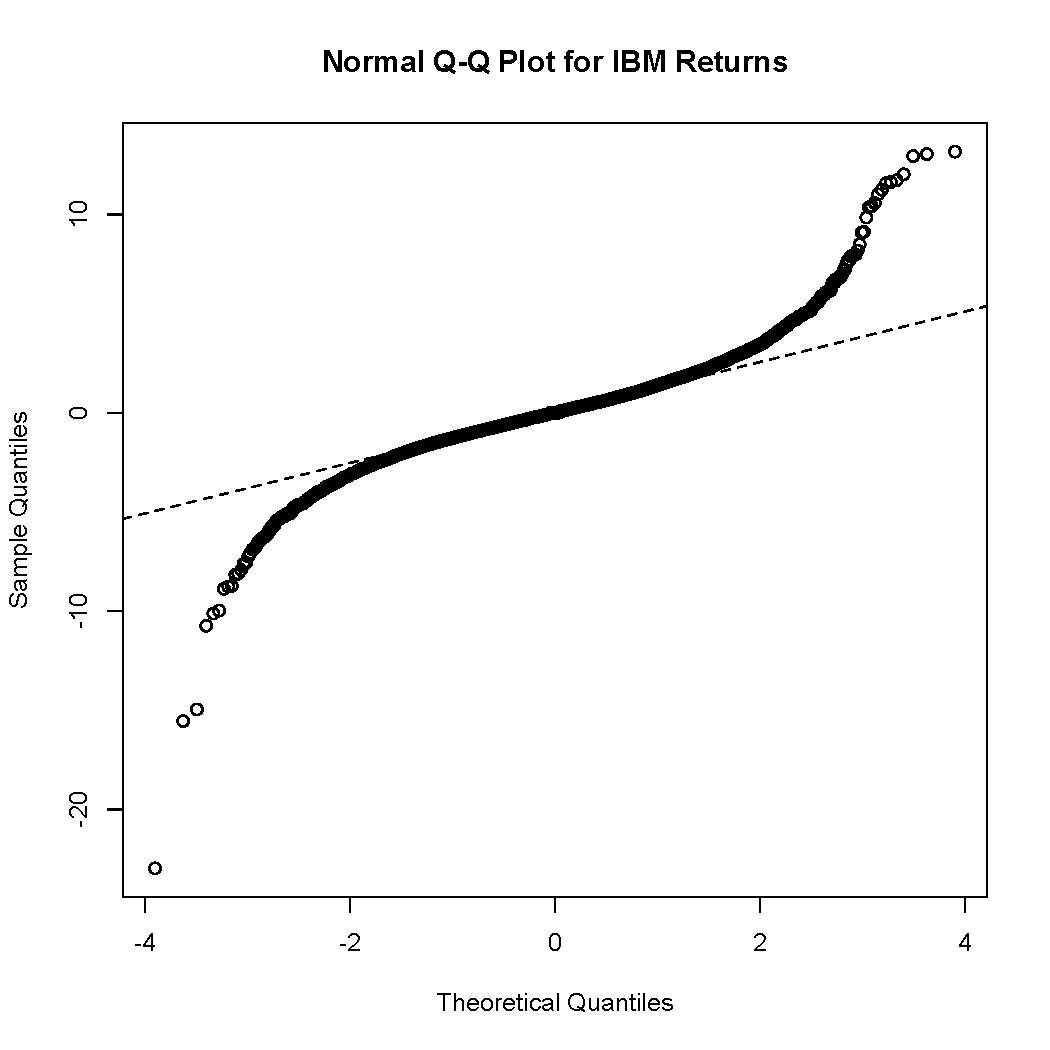
\includegraphics[scale=.5]{ibm-qq}
  \caption[Q-Q Plot of Returns]{By looking at a quantile-quantile plot of our data set, we see that returns are not normally distributed. The tails deviate sharply from normality.}
  \label{figure:ibm-qq}
\end{figure}

\index{R language} 
\begin{verbatim}
rets<-read.table("d-ibmvwewsp6203")
attach(rets)
retsts<-ts(V2,start=c(1962,190),frequency=260)
plot(retsts,ylab="IBM Returns", typ="p") 

qqnorm(V2,main="Normal Q-Q Plot for IBM Returns")
qqline(V2,lty=2)
\end{verbatim}

\begin{figure}[tb]
  \centering
  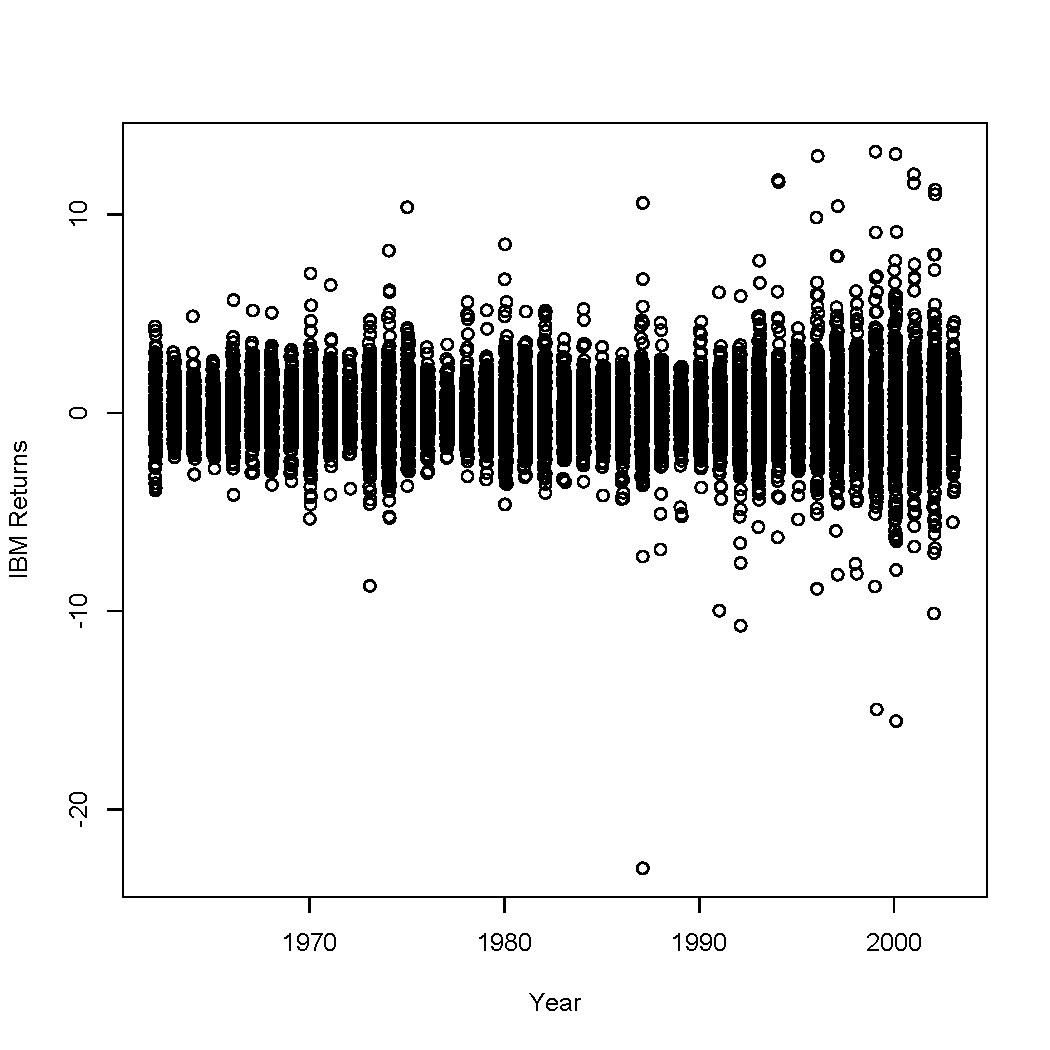
\includegraphics[scale=.5]{ibm-ret}
  \caption[IBM Returns]{IBM returns become more varied over time, deviating further from zero.}
  \label{figure:ibm-ret}
\end{figure}

\paragraph{Normal Distribution.} For the sake of simplicity, returns are often considered to be \emph{\mbox{normally} distributed}. However, the lower bound of a simple is -1, total loss of the asset. The normal distribution has no lower bound. Also, multiperiod returns (\emph{the product of one-period \mbox{returns}, \eqref{eq:multiperiod} is a multiperiod return}) of a normally distributed returns are themselves not normally distributed. Additionally, asset returns observed in reality have positive excess kurtosis, and do not fit the normal distribution.

\paragraph{Lognormal Distribution.} Instead of assuming a normal distribution, we could assume that the log returns $r_t$ of an asset are independent and identically distributed (\emph{iid})\index{iid -- independent and\\identically distributed} as normal with mean $\mu$ and variance $\sigma^2$, which makes simple returns iid\index{iid -- independent and\\identically distributed} lognormal random variables, and mean and variance are,
\[
E(R_t)=\exp \left( \mu + \frac{\sigma^2}{2} \right) -1, \quad
\text{Var}(R_t) = \exp(2\mu+\sigma^2)[\exp(\sigma^2)-1].
\]
The mean and variance of the log returns $r_t$ when $m_1$ and $m_2$ are the mean and variance of the simple return $R_t$
\[
E(r_t) = \ln \left( \frac{m_1+1}{\sqrt{1+m_2 / (1+m_1)^2}} \right), \quad
\text{Var}(r_t)=\ln \left( 1+\frac{m_2}{(1+m_1)^2} \right).
\]
$Y$ is lognormal if $X = \ln(Y)$ is normal.

\subsection{Power Generation and Delivery Time Series}
As a practical example of \fts{}, we will briefly focus on power generation and delivery -- the route that electricity makes in its supply chain from fuel to its consumption in homes and businesses. Electricity demand is contingent upon weather, among other factors. Likewise, the supply of electricity requires consideration of many time series.

Some background reading to understand the power generation and delivery fundamentals are at the EIA website., ``How is my electricity generated, delivered, and priced?''\footnote{The U.S. Energy Information Administration publishes detailed statistics and news regarding energy production and consumption on it web site \texttt{http://www.eia.doe.gov}. A good introduction to electricity generation is at  \texttt{http://tonto.eia.doe.gov/energy\_in\_brief/electricity.cfm}}.

\paragraph{Generation.} When considering how electricity is generated, we must consider sources of generation,
\begin{enumerate}
	\item coal
	\item natural gas
	\item nuclear
	\item hydroelectric
	\item wind
	\item others \ldots
\end{enumerate}
Some of these source require a fuel source to create heat, which boils water to create steam to turn electricity-generating turbines. Clearly, our analysis of \fts{} should include inputs like fuel costs.

Power plants cannot operate every minute of every day. There will be times that require maintenance or refueling. The time to perform these tasks might be several weeks, and some outages are planned, others are unplanned. For this reason, multiple power stations will be generating concurrently. This is also a factor that must considered when modeling the generation of power.

\paragraph{Delivery.} Electricity, when generated at a power plant, must be transmitted distances to areas for local consumption. There is only so much power that can travel across high-voltage lines at any given time. When demand is very high, the transmission lines reach a point of \emph{congestion}. When this occurs, the best route through which to deliver power must be obtained very quickly.

\subsubsection{Weather}
Performing quantitative weather prediction uses current weather conditions as an input into mathematical models of the atmosphere to predict temperature and rainfall.
\margincomment{Computer models forecast changes in temperature and rainfall.}
These predictions are important to power generation and delivery because electricity demand has some relationship to the current temperature. Power sources such as hydroelectric and wind require plenty of upstream water and winds to produce electricity.

Due to the complex nature of weather modeling, it is only feasible to create any reliable and timely forecasts in real-time with advanced computing technology. The task requires manipulating very large datasets and performing complex calculations. Using \emph{ensemble forecasts}\index{ensemble forecasts} helps us to define the forecast uncertainty and extend weather forecasting farther into the future than would otherwise be possible.

A model, in this context, is a computer program that produces meteorological information for future times at given positions and altitudes. The horizontal domain of a model is either global, covering the entire Earth, or regional, covering only part of the Earth. Regional models also are known as limited-area models.

The forecasts are computed using mathematical equations for the physics and dynamics of the atmosphere. These equations are \emph{nonlinear} and are impossible to solve exactly.
\margincomment{Numerical forecast methods obtain approximate solutions.} Different models use different solution methods. Global models often use \emph{spectral methods}\index{spectral methods} for the horizontal dimensions and finite difference methods for the vertical dimension, while regional models usually use finite-difference methods in all three dimensions. Regional models also can use finer grids to explicitly resolve smaller-scale meteorological phenomena, since they do not have to solve equations for the whole globe. We discuss examples of spectral methods in Section~\ref{spectral methods}.

Models are initialized using observed data from weather satellites and surface weather observation stations. The irregularly-spaced observations are processed by data assimilation and objective analysis methods, which perform quality control and obtain values at locations usable by the model's mathematical algorithms (usually an evenly-spaced grid). The data are then used in the model as the starting point for a forecast. Commonly, the set of equations used is known as the \emph{primitive equations}. These equations are initialized from the analysis data and rates of change are determined. The rates of change predict the state of the atmosphere a short time into the future.

The equations are then applied to this new atmospheric state to find new rates of change, and these new rates of change predict the atmosphere at a yet further time into the future.
\margincomment[red]{Most time series analysis assumes evenly-spaced observations. We cannot make that assumption in weather modeling.}
This time stepping procedure is continually repeated until the solution reaches the desired forecast time. The length of the time step is related to the distance between the points on the computational grid. Time steps for global climate models may be on the order of tens of minutes, while time steps for regional models may be a few seconds to a few minutes.

\paragraph{Ensemble Forecasts.} Long-range weather forecasting requires the application of some theory taken from fluid dynamics \cite{lorenz1969pfp}. Ensembles were proposed by Edward Lorenz\index{Lorenz, Edward} in an attempt to make extended forecasts despite the chaotic nature of the fluid dynamics equations required. There is tremendous amounts of uncertainty during the path of a weather pattern, which covers thousands of miles. To account for this uncertainty, stochastic or ``ensemble" forecasting is used, involving multiple forecasts created with different model systems, different physical parametrizations, or varying initial conditions. The ensemble forecast is usually evaluated in terms of the ensemble mean of a forecast variable, and the ensemble spread, which represents the degree of agreement between various forecasts in the ensemble system, known as ensemble members.

\subsubsection{Fuel Prices}
In most cases, to generate electricity at a power plant, we require a fuel of some kind. That fuel may be coal, natural gas, or nuclear fuel such as uranium. The price to purchase and receive for delivery these fuels is affected by market forces.

\paragraph{Natural Gas.}
One of the most abundant fuel sources for power generation is natural gas. The contracts for delivery have different terms, and delivery points throughout North America \cite[p.3--5]{eydeland-wolyniec2002}.
\begin{itemize}
	\item\index{natural gas delivery!baseload firm}\index{baseload firm|see{natural gas delivery}}{\textbf{Baseload Firm}. In this transaction, the delivering party is expected to perform according to the contract under most any conditions.}
	\item\index{natural gas delivery!baseload interruptible}\index{baseload interruptible|see{natural gas delivery}}{\textbf{Baseload Interruptible}. Delivery can be interrupted, and the conditions may or may not be specific in the contract.}
	\item\index{natural gas delivery!swing}\index{swing|see{natural gas delivery}}{\textbf{Swing}. The volume of delivered gas is adjusted daily at the buyer's discretion, typically for daily pipeline volume balancing.}
\end{itemize}

\paragraph{Transportation.}
Contractual provisions of natural gas delivery may vary.
\begin{itemize}
	\item\index{natural gas transportation!firm transportation service}{\textbf{Firm Transportation Service}. Firm transportation service is the highest priority service.}
	\item\index{natural gas transportation!interruptible transportation contract}{\textbf{Interruptible Transportation Contract}. A pipeline has an option to interrupt the service on short notice without a penalty.}
\end{itemize}

\subsubsection{Electricity Delivery Capacity}
\paragraph{Energy Markets.}
In order to coordinate delivery across state boundaries and to ensure competitive power markets, there are independent system operators\index{independent system operator} (``ISO") and regional transmission organizations\index{regional transmission organization} (``RTO"). One example of an RTO is the \emph{PJM Interconnection} which has the task of coordinating the continuous buying, selling and delivery of wholesale electricity throughout the Pennsylvania, New Jersey, and Maryland area, as well as parts of Illinois, Indiana, Michigan. In its role as market operator, PJM balances the needs of suppliers, wholesale customers and other market participants and monitors market activities to ensure open, fair and equitable access.

PJM operates much like an exchange, with market participants establishing prices for electricity by matching supply and demand. The market uses \emph{locational marginal pricing}\index{locational marginal pricing} (LMP) that reflects the value of the energy at the specific location and time it is delivered. If the lowest-priced electricity can reach all locations, prices are the same across the entire grid. When there is transmission congestion, energy cannot flow freely to certain locations. In that case, more-expensive electricity is ordered to meet that demand. As a result, the locational marginal price is higher in those locations.

The energy market consists of \emph{day-ahead} and \emph{real-time} markets. The Day-Ahead Market is a forward market in which hourly LMPs are calculated for the next operating day based on generation offers, demand bids and scheduled bilateral transactions. The real-time Market is a spot market in which current LMPs are calculated at five-minute intervals based on actual grid operating conditions. Real-time prices are available. An RTO settles transactions hourly and issues invoices to market participants monthly.

\paragraph{Electricity Prices.} Electricity prices tend to experience abrupt price spikes\index{price spikes}, which are very short-term price increases of unpredictable magnitude \cite[p. 25]{weron2006mfel}\footnote{A good introduction to energy trading is \citeA{fusaro1998erm}. Although a bit dated by now, it contains some important fundamentals of the fuel markets. Further detail on price and volatility modeling can be found in \citeA{pilipovic2007er}.}.
\margincomment[red]{Electricity prices are extremely volatile, but follow a seasonal pattern.}
Because of these spikes, measuring the volatility of electricity prices is an important issue. Additionally, electricity demand tends to fluctuate seasonally, and we should expect its price to follow that pattern in some way.

Price volatility is not a single number, but rather, an array of numbers through time. How much fluctuation is observed in electricity prices to be delivered in ten minutes will not have the same fluctuation as that delivered in an hour, or a week from now. To represent this array, we require a \emph{term structure of volatility}\index{term structure of volatility} \cite[p. 328]{harris2006em},
\begin{equation}
\sigma_{a,T,t} = \Bigg( \frac{1}{(T-t)} \int^T_t \sigma^2(s)ds \Bigg)^{0.5}
\label{eq:tsov}
\end{equation}
where $T$ is the contract delivery date and $t$ is the observation date.

We shall see in Section~\ref{garch-spec} and in Section~\ref{crosscorrmatr} how to implement the term structure in \eqref{eq:tsov} to create volatility models. Using power generation and delivery as one example of a market with several kinds of \fts{}, we can further explore the numerical methods that give us insight into the markets themselves.